\chapter{Cold free fermion neutron stars}
\label{chap:nstars}

\TODO{better title}

\TODO{references}

\TODO{intro}

In \cref{chap:tft}, we found $Z = Z(T, \mu, V)$ for two sample systems, and in particular a gas of free Dirac fermions.
From $Z$, we can derive the pressure $P = P(T, \mu)$ and energy density $\epsilon = \thermalavg{E}/V = \epsilon(T, \mu)$ using \cref{eq:tft:average_number,eq:tft:average_energy,eq:tft:average_pressure}, where the volume $V$ has been eliminated by division, because $P$ and $\epsilon$ are intensive quantities.
At some fixed temperature $T$, we can therefore eliminate $\mu$ to express $\epsilon$ in terms of $P$.
This gives us an equation of state $\epsilon = \epsilon(P)$ with which we can solve the Tolman-Oppenheimer-Volkoff system \eqref{eq:tov:tovsys}.

In this chapter, we will use partition function \eqref{eq:tft:dirac_partition_function} for free Dirac fermions and do exactly this to model a neutron star with a cold ideal Fermi gas of neutrons.
\TODO{bad wording: use something like ``equation of state for free/ideal cold fermi gas?}

\textit{This chapter is inspired by references \cite{ref:jensoluf}, \cite{ref:glendenning}, \cite{ref:mtw} and \cite{ref:stability_methods}.}

\section{Equation of state}

For easy reference, the logarithm of the free Dirac fermion partition function \eqref{eq:tft:dirac_partition_function} is
\begin{equation}
	\log Z = 2 V \int \frac{\dif^3 p}{(2 \pi \hbar)^3} \bigg\{ \beta E(\vec{p}) + \log \left[ e^{-\beta (E(\vec{p}) - \mu)}+1 \right] + \log \left[ e^{-\beta (E(\vec{p}) + \mu)} + 1\right] \bigg\}.
\end{equation}
First, the particle number density $n = \thermalavg{N}/V$ follows from the derivative \eqref{eq:tft:average_number} and is
\begin{equation}
	n = 
	\frac{1}{\beta} \pdv{\log Z}{\mu} =
	2 \int \frac{\dif^3 p}{(2 \pi \hbar)^3} \Big\{ n\big[ E(\vec{p})-\mu \big] - n\big[ E(\vec{p})+\mu \big] \Big\} ,
\label{eq:nstars:density}
\end{equation}
where we defined the \textbf{Fermi-Dirac distribution} \TODO{plus or minus in exponential?}
\begin{equation}
	n(E) = \frac{1}{e^{-\beta E} + 1}.
\label{eq:nstars:fermi_dirac_distribution}
\end{equation}
Do not confuse the particle density $n$ on the left with the Fermi-Dirac distributions $n[E(\vec{p}) \mp \mu]$ on the right!
We will soon perform the integral over $\vec{p}$ and get rid of $n[E(\vec{p}) \mp \mu]$, anyway.
From the density \eqref{eq:nstars:density}, we see that $n = n(\mu, T)$ is a function of the chemical potential $\mu$ and temperature $T$, so that at some fixed temperature, the value of $\mu$ determines the particle density $n$.

Second, we calculate the energy density $\epsilon = \thermalavg{E} / V$ from \cref{eq:tft:average_energy}.
Inserting the particle number density \eqref{eq:nstars:density} and taking the derivative of $\log Z$, we get
\begin{equation}
	\epsilon = 
	\mu n - \frac{1}{V} \pdv{\log Z}{\beta} =
	2 \int \frac{\dif^3 p}{(2 \pi \hbar)^3} \Big\{ -E(\vec{p}) + E(\vec{p}) \, n\big[ E(\vec{p})-\mu \big] + E(\vec{p}) \, n\big[ E(\vec{p})+\mu \big] \Big\}.
\label{eq:nstars:energy_density}
\end{equation}

Third, we find that the pressure \eqref{eq:tft:average_pressure} is
\begin{equation}
	P =
	\frac{\log Z}{\beta V} = 
	2 \int \frac{\dif^3 p}{(2 \pi \hbar)^3} \bigg\{ E(\vec{p}) + \log \left[ e^{-\beta(E(\vec{p})-\mu)} + 1 \right] + \log \left[ e^{-\beta(E(\vec{p})+\mu)} + 1 \right] \bigg\}.
\label{eq:nstars:pressure}
\end{equation}

The first term of the energy density \eqref{eq:nstars:energy_density} and the pressure \eqref{eq:nstars:pressure} is infinite, as the integrand never decays \TODO{decay usually associated with radiation}.
This can be interpreted as an infinite shift of the vacuum energy.
In contrast, the two last terms are finite as the integrand is suppressed \TODO{?} for large $\abs{\vec{p}}$ by the Fermi-Dirac distribution.
It makes no sense to include a term that integrates over every possible value of the momentum $\vec{p}$ for physical particles whose momentum cannot exceed a certain value due to energy conservation.
Here, we will make the assumption that we can simply drop the infinite term.
We will return later to investigate this term by regularization and renormalization. \TODO{does this make sense?} \TODO{improve convergence/divergence arguments, look at measure $p^2$, etc.}

From the particle density \eqref{eq:nstars:density} at constant temperature $T$, we see that the sign of $n$ is determined by the sign of $\mu$.
The total density $n$ is expressed as a balance between \emph{particles} with energy $E(\vec{p}) > 0$ living relative to the chemical potential $\mu$ and \emph{antiparticles} with energy $E(\vec{p}) < 0$ living relative to the chemical potential $-\mu$.
Thus, the chemical potential $\mu$ determines the balance between particles and antiparticles in the system.
Similarly, the two last terms in the energy density \eqref{eq:nstars:energy_density} and pressure \eqref{eq:nstars:pressure} can be interpreted as contributions from particles and antiparticles.
We choose a large, positive value of $\mu > 0$, so that the particles dominate the system, while antiparticles are hardly present.
With this choice, $n \left[ E(\vec{p}) - \mu \right] \gg n \left[ E(\vec{p}) + \mu \right]$, and we drop the last term from the particle density \eqref{eq:nstars:density}, energy density \eqref{eq:nstars:energy_density} and pressure \eqref{eq:nstars:pressure}.

Dropping terms as described in the last paragraphs, we are left with the%
\begin{subequations}%
\begin{align}%
	& \text{particle density} & n        &=  2 \int \frac{\dif^3 p}{(2 \pi \hbar)^3} \, n \left[ E(\vec{p})-\mu \right] ,                    \label{eq:nstars:dropped_infinities_density} \\
	& \text{energy density}   & \epsilon &=  2 \int \frac{\dif^3 p}{(2 \pi \hbar)^3} \, E(\vec{p}) \, n \left[ E(\vec{p})-\mu \right] ,      \label{eq:nstars:dropped_infinities_energy_density} \\
	& \text{pressure}         & P        &= -2 \int \frac{\dif^3 p}{(2 \pi \hbar)^3} \, \log \left[ e^{-\beta(E(\vec{p})-\mu)} + 1 \right] . \label{eq:nstars:dropped_infinities_pressure}
\end{align}%
\label{eq:nstars:dropped_infinities}%
\end{subequations}%
The integrals become nasty after plugging in the relativistic dispersion relation \eqref{eq:tft:dispersion} and the Fermi-Dirac distribution \eqref{eq:nstars:fermi_dirac_distribution}, and it is overly optimistic to expect that all of them can be evaluated analytically.
We will make one final approximation that will make all the integrals surmountable.

At \emph{absolute} zero temperature $T = 0$, the Fermi-Dirac distribution
\begin{equation}
	n(E) = \frac{1}{e^{\beta (E - \mu)} + 1} = \theta(\mu-E) = \begin{cases} 0 & (E > \mu) \\ 1 & (E < \mu) \end{cases}
\end{equation}
behaves like a step function.
To see this, observe that $T = 0$ corresponds to $\beta = \infty$, and that the sign of $E - \mu$ determines whether the exponential $e^{\beta (E - \mu)}$ in the denominator blows up or vanishes, and hence whether the fraction survives.
Physically, this means that the system is completely degenerate, filling momentum states with $E(\vec{p}) < \mu$ only.
The filled states with highest momentum $p_F$ make up a so-called \emph{Fermi surface} $\abs{\vec{p}} = p_F$ in momentum space, and the corresponding maximum energy $E_F = \sqrt{p_F^2 c^2 + m^2 c^4}$ is called the \emph{Fermi energy}, and is equal to the chemical potential when $T = 0$.

Typical neutron star core temperatures linger around $T_0 \approx \SI{1e6}{\kelvin}$, \cite{ref:glendenning} so how is this relevant for our purposes?
By using a Sommerfeld expansion, it is possible to show mathematically that the chemical potential at a finite temperature $T > 0$ is corrected from the Fermi energy by
\cite[section 3.6]{ref:notes_statistical_physics_tong}, \cite[exercise 2]{ref:eth_statistical_physics_exercise}
\begin{equation}
	\mu(T) = E_F + \bigo \left( \left( \frac{T}{T_F} \right)^2 \right) ,
	%\mu(T) = E_F - \frac{\pi^2}{6} (k_B T)^2 \frac{g'(E_F)}{g(E_F)}
\end{equation}
to first nonzero order in $T/T_F$, where $T_F = E_F / k_B$ is the \emph{Fermi temperature} corresponding to the Fermi energy $E_F$, and $g(E)$ the density of states.
Neutrons have mass $m \approx \SI{1.67e-27}{\kilogram}$, so $T_F = \sqrt{p_F^2 c^2 + m^2 c^4} / k_B > m c^2 / k_B \approx \SI{1e13}{\kelvin}$.
Thus, $T / T_F < T_0 / T_F \approx 10^{-7} \ll 1$, and it is therefore an excellent approximation to take the limit
\begin{equation}
	\beta \mu \gg 1 .
\end{equation}
By rewriting the Fermi-Dirac distribution as
\begin{equation}
	n(E) = \frac{1}{e^{\beta \mu (E/\mu - 1)} + 1} ,
\label{eq:nstars:zero_temperature_limit}
\end{equation}
we can again see that in the zero-temperature limit \eqref{eq:nstars:zero_temperature_limit}, the sign of $E - \mu$ will again force the distribution into a simple step function, as at absolute zero temperature.
Thus, the zero-temperature behavior of the Fermi-Dirac distribution is restored in this limit.
Although the temperature itself is far from zero, this approximation is therefore referred to as the \textbf{zero-temperature approximation}.

Alternatively, since the chemical potential is an independent variable in the partition function, we could simply have \emph{assumed} the zero-temperature limit \eqref{eq:nstars:zero_temperature_limit} when we said we \emph{chose} a ``large, positive value'' for the chemical potential.

\iffalse
\begin{figure}
	\centering
	\begin{tikzpicture}
		\begin{groupplot}[group style={group size=2 by 1, horizontal sep=5pt}, height=6cm, width=7cm, /tikz/declare function={
			n(\b,\E) = 1/(exp(\b*\E)+1);
		}]
			\nextgroupplot[xlabel=$E$, ylabel=$1/(e^{\beta E}+1)$, 
				colorbar horizontal, colorbar sampled, colorbar style={xlabel=$\beta$, samples=7, xtick={-0.5, 0.5, 1.5, 2.5, 3.5, 4.5}, xticklabels={$1/2$, $1$, $2$, $4$, $8$, $16$, $32$}, grid=none, xticklabel pos=upper, tickwidth=0, at={(0.0,1.03)}, anchor=south west},
				every colorbar/.append style={width=2*\pgfkeysvalueof{/pgfplots/parent axis width}+\pgfkeysvalueof{/pgfplots/group/horizontal sep}},
				xtick distance=10, ytick distance=0.5, grid=none, minor tick num=1,
			]
			\pgfplotsinvokeforeach{0.5, 1, 2, 4, 8, 16, 32}{
				\addplot[domain=-10:+10, samples=200, mesh, point meta={log2(#1)}] {n(#1, x)};
			}

			\nextgroupplot[xlabel=$E$, ylabel=$\log (e^{-\beta E}+1)/\beta$, xtick distance=10, yticklabel pos=right, ytick distance=5, minor tick num=1, grid=none]
			\pgfplotsinvokeforeach{0.5, 1, 2, 4, 8, 16, 32}{
				\addplot[domain=-10:+10, samples=200, mesh, point meta={log2(#1)}] {ln(exp(-#1*x)+1)/#1};
			}
		\end{groupplot}
	\end{tikzpicture}
\caption{\label{fig:nstars:distribution_convergence}%
	In the zero-temperature limit $\beta E \gg 1$, the Fermi-Dirac distribution $1/(e^{\beta E}+1) \rightarrow \theta(-E)$, while $\log (e^{-\beta E} + 1) \rightarrow -\beta E \, \theta(-E)$, where $\theta(E)$ is the step function.
}
\end{figure}
\fi

In the zero-temperature limit, the Fermi-Dirac distribution can be replaced by
\begin{equation}
	n(E)       =                 \begin{cases} 1 / (e^{+\beta \abs{E}}+1) & (E>0) \\ 1 / (e^{-\beta \abs{E}}+1) & (E<0) \end{cases}
	     \quad \rightarrow \quad \begin{cases} 0 & (E>0) \\ 1 & (E<0) \end{cases}
	     \quad =                 \theta(-E) ,
\end{equation}
while the logarithm in the pressure behaves as
\begin{equation}
	\log (e^{-\beta E}+1)       =                 \begin{cases} \log (e^{-\beta \abs{E}}+1) & (E>0) \\ \log (e^{+\beta \abs{E}}+1) & (E<0) \end{cases}
	                      \quad \rightarrow \quad \begin{cases} \log 1 & (E>0) \\ \log e^{-\beta E} & (E<0) \end{cases}
	                      \quad =                 -\beta E \, \theta(-E) .
\end{equation}
This is confirmed by the plots in \cref{fig:nstars:distribution_convergence} for increasing values of $\beta$.
Thus, the zero-temperature limit effectively limits the integrals \eqref{eq:nstars:dropped_infinities} to those momenta $\vec{p}$ with $E(\vec{p}) < \mu$.
We therefore call
\begin{equation}
	\mu = E_F = E(p_F) = \sqrt{p_F^2 c^2 + m^2 c^4}
\end{equation}
the Fermi energy and the corresponding momentum $p_F$ the Fermi momentum, representing the occupied state in momentum-space with largest energy and momentum.

Now the particle density \eqref{eq:nstars:dropped_infinities_density} simply becomes
\begin{equation}
	n = 
	2 \int_0^\infty \frac{\dif p \, 4 \pi p^2}{(2 \pi \hbar)^3} \theta \left[ \mu - E(p) \right] =
	2 \int_0^{p_F} \frac{\dif p \, 4 \pi p^2}{(2 \pi \hbar)^3} = \frac{p_F^3}{3 \pi^2 \hbar^3} .
\label{eq:nstars:density_zeroT}
\end{equation}
Using integral \TODO{ref} and defining the dimensionless momentum $x = p / mc$, the energy density \eqref{eq:nstars:dropped_infinities_energy_density} is
\begin{equation}
\begin{split}
	\epsilon &=  2 \int_0^\infty \frac{\dif p \, 4 \pi p^2}{(2 \pi \hbar)^3} \, E(p) \, \theta \left[ \mu - E(p) \right] \\
	         &=  2 \int_0^{p_F} \frac{\dif p \, 4 \pi p^2}{(2 \pi \hbar)^3} \, \sqrt{p^2 c^2 + m^2 c^4} \\
	         &= \frac{m^4 c^5}{\pi^2 \hbar^3} \int_0^{x_F} \dif x \, x^2 \sqrt{1 + x^2} \\
	         &= \frac{m^4 c^5}{8 \pi^2 \hbar^3} \left[ \left( 2 x_F^3 + x_F \right) \sqrt{1 + x_F^2} - \asinh x_F \right] . \\
\end{split}
\label{eq:nstars:energy_density_zeroT}
\end{equation}
Finally, using the same integral, the pressure \eqref{eq:nstars:dropped_infinities_pressure} is
\begin{equation}
\begin{split}
	P &= \frac{2}{\beta} \int_0^\infty \frac{\dif p \, 4 \pi p^2}{(2 \pi \hbar)^3} \, \beta \left[ \mu - E(p) \right] \, \theta \left[ \mu - E(p) \right] \\
	  &= 2 \int_0^{p_F} \frac{\dif p \, 4 \pi p^2}{(2 \pi \hbar)^3} \, \left[ \sqrt{p_F^2 c^2 + m^2 c^4} - \sqrt{p^2 c^2 + m^2 c^4} \right] \\
	  &= \frac{m^4 c^5}{\pi^2 \hbar^3} \int_0^{x_F} \dif x \, x^2 \left[ \sqrt{x_F^2+1} - \sqrt{x^2+1} \right] \\
	  &= \frac{m^4 c^5}{24 \pi^2 \hbar^3} \left[ \left( 2 x_F^3 - 3 x_F \right) \sqrt{x_F^2 + 1} + 3 \asinh x_F \right] . \\
\end{split}
\label{eq:nstars:pressure_zeroT}
\end{equation}

The equation of state $\epsilon = \epsilon(P)$ follows by eliminating $x_F$ from the energy density \eqref{eq:nstars:energy_density_zeroT} and pressure \eqref{eq:nstars:pressure_zeroT}.
Due to their complicated dependence on $x_F$, we will do so in three cases of increasing difficulty.

\TODO{first present three cases, \emph{then} do calculations, to not overload the reader}

\subsection{Ultra-relativistic limit}
\label{sec:nstars:ur_limit}

First, consider the ultra-relativistic limit
\begin{equation}
	x_F \gg 1 , 
\label{eq:nstars:ur_limit}
\end{equation}
where the Fermi energy $E_F = \sqrt{p_F^2 c^2 + m^2 c^4} \taylor p_F c$ is dominated by the contribution from the Fermi momentum.
Since $\asinh x_F = \log \left[ x_F + \sqrt{x_F^2 + 1} \right] \taylor \log 2 x_F$ diverges logarithmically, we see that both the energy density \eqref{eq:nstars:energy_density_zeroT} and pressure \eqref{eq:nstars:pressure_zeroT} are dominated by their first term with $2 x_F^3 \sqrt{x_F^2 + 1} \taylor 2 x_F^4$.
In the ultra-relativistic limit, then,
\begin{equation}
	\epsilon \taylor \frac{m^4 c^5 x_F^4}{4 \pi^2 \hbar^3}
	\qquad \text{and} \qquad
	P        \taylor \frac{m^4 c^5 x_F^4}{12 \pi^2 \hbar^3},
\end{equation}
and $x_F$ is easily eliminated, yielding the very simple equation of state
\begin{equation}
	\epsilon = 3 P .
\label{eq:nstars:ur_eos}
\end{equation}

In this particular case, the TOV system \eqref{eq:tov:tovsys} can be solved analytically with the polynomial trial solution
\begin{equation}
	P(r) = A r^n .
\label{eq:nstars:ur_ansatz}
\end{equation}
Then the mass equation \eqref{eq:tov:tovsys_mass} is
\begin{equation}
	\odv{m}{r} = \frac{12 \pi A}{c^2} r^{n+2},
	\qquad \text{so} \qquad
	m(r) = \frac{12 \pi A}{(n+3) c^2} r^{n+3}
	\quad (n \neq -3).
\label{eq:nstars:ur_mass}
\end{equation}
With the equation of state \eqref{eq:nstars:ur_eos}, mass \eqref{eq:nstars:ur_mass} and trial solution \eqref{eq:nstars:ur_ansatz}, the TOV equation \eqref{eq:tov:tovsys_pressure} reads
\begin{equation}
	n A r^{n-1} =
	-\frac{48 \pi G A^2 r^{2n+1}}{(n+3) c^4} \left[ 2 + \frac{n}{3} \right] \left[ 1 - \frac{24 \pi G A r^{n+2}}{(n+3) c^4} \right]^{-1} .
\end{equation}
We can attain equality for all $r$ if we choose $n = -2$.
Then the rightmost factor no longer depends on $r$, and both sides have the same $r^{-3}$-dependence
\begin{equation}
	- 2 A r^{-3} = - \frac{64 \pi G A^2 r^{-3}}{c^4} \left[ 1 - \frac{24 \pi G A}{c^4} \right]^{-1} .
\end{equation}
Equality is established if we match the prefactors by choosing $A = c^4 / 56 \pi G$.
Then the solutions for the pressure and mass are
\begin{equation}
	P(r) = \frac{c^4}{56 \pi G} \frac{1}{r^2}
	\qquad \text{and} \qquad
	m(r) = \frac{3 c^2}{14 G} r .
\end{equation}
This is a highly unphysical result.
The pressure diverges at the center, so nothing could ever hold such a star together.
In addition, $p(r) > 0$ for all $r$, so the star has no surface and hence infinite mass $M = m(\infty) = \infty$.

\TODO{make plot of $P(r)$ and $m(r)$ for a star.}

\subsection{Non-relativistic limit}
\label{sec:nstars:nr_limit}

Next, let us consider the more difficult non-relativistic limit
\begin{equation}
	x_F \ll 1,
\label{eq:nstars:nr_limit}
\end{equation}
where the Fermi energy $E_F = \sqrt{p_F^2 c^2 + m^2 c^4} \taylor m c^2$ is dominated by the rest energy of the fermions.
Taylor expanding the energy density \eqref{eq:nstars:energy_density_zeroT} and presure \eqref{eq:nstars:pressure_zeroT} around $x_F = 0$ to lowest order, we find
\begin{equation}
	%\epsilon &\taylor \frac{m c^2 p_F^3}{3 \pi^2 \hbar^3} + \frac{p_F^5}{10 \pi^2 \hbar^3 m} = n m c^2 + \frac{p_F^5}{10 \pi^2 \hbar^3 m} \\
	%P        &\taylor \frac{p_F^5}{15 \pi^2 \hbar^3 m}
	\epsilon \taylor \frac{m c^2 p_F^3}{3 \pi^2 \hbar^3}
	\qquad \text{and} \qquad
	P        \taylor \frac{p_F^5}{15 \pi^2 \hbar^3 m} .
\end{equation}
Note that with the density \eqref{eq:nstars:density}, the energy density can be written $\epsilon = n m c^2$, so it is only due to the rest mass of the particles, as if all fermions have broken free from the Pauli exclusion principle and possess the same rest energy $m c^2$.
This is only a mathematical feature of the non-relativistic limit -- the fermions still occupy different states with different momentum, but the momenta are so small that the differences are negligible compared to the rest energy $mc^2$.
Again, it is straightforward to eliminate $x_F$ to find the equation of state, only this time there is some extra bookkeeping with all the exponents.
Carefully gathering all the prefactors under the same roof, we find
\begin{equation}
	%\epsilon = \frac{mc^2}{3\pi^2\hbar^3} \left( 15 \pi^2 \hbar^3 m P \right)^{3/5}
	\epsilon = \left( \frac{5^3 m^8 c^{10}}{3^2 \pi^4 \hbar^6} \right)^{\frac15}  P^{\frac35} .
\label{eq:nstars:nr_eos}
\end{equation}
With this power dependence, it is not easy, if even possible, to solve the TOV equation analytically.
The trial solution \eqref{eq:nstars:ur_ansatz} we employed in \cref{sec:nstars:ur_limit} fails miserably, as we do not get the same fortunate cancellations of $r$.
We therefore resort to the numerical solution method described in \cref{sec:nstars:numtov}, parametrizing different stars by their central pressure $P_0$ and integrating the TOV equation until the pressure $p(R)$ vanishes, using the corresponding radius $R$ to establish the mass $M = m(R)$ of the star.
The results are shown in \cref{fig:nstars:massradius}.

\TODO{compare with earlier results, most massive neutron stars}

\iffalse
Dimensionless equation of state
\begin{equation}
	\diml{\epsilon} = \left[ \frac{4^2 5^3}{3^4 \pi^2} \frac{m^8 c^6 r_0^6}{m_0^2 \hbar^6} \diml{P}^3 \right]^{\frac{1}{5}}
\end{equation}
\fi

\subsection{General Fermi momenta}
\label{sec:nstars:gr_limit}

How can we find the energy density
\begin{equation}
	\epsilon = \frac{m^4 c^5}{8 \pi^2 \hbar^3} \left[ \left( 2 x_F^3 + x_F \right) \sqrt{1 + x_F^2} - \asinh x_F \right]
\label{eq:nstars:gr_limit_energy_density}
\end{equation}
that corresponds to a given pressure
\begin{equation}
	P = \frac{m^4 c^5}{24 \pi^2 \hbar^3} \left[ \left( 2 x_F^3 - 3 x_F \right) \sqrt{x_F^2 + 1} + 3 \asinh x_F \right] 
\label{eq:nstars:gr_limit_pressure}
\end{equation}
for general $x_F$?
Since we are already solving the TOV equation on a computer, we can do so by numerical root finding.
At every step $r$ in the numerical integration algorithm, we know the current pressure $P = P(r)$.
Using a numerical root finding algorithm, we can find the root $x_F$ of the function
\begin{equation}
	f(x_F) = P(x_F) - P = 0,
\end{equation}
where $P(x_F)$ is the pressure \eqref{eq:nstars:gr_limit_pressure} as a function of $x_F = p_F / m c$.
Having found the root, we can simply calculate the corresponding energy density $\epsilon(x_F)$ from \cref{eq:nstars:gr_limit_energy_density}.
This whole procedure can be elegantly encapsulated into a function that implements an implicit equation of state $\epsilon = \epsilon(P)$, which in turn is straightforward to plug into our solver described in \cref{sec:nstars:numtov}.
The results are shown in \cref{fig:nstars:massradius}.

\iffalse
\begin{equation}
	\diml{P}(x_F) = \frac{m^4 c^3 r_0^3}{18 \pi m_0 \hbar^3} \left[ (2 x_F^3 - 3 x_F) \sqrt{x_F^2 + 1} + 3 \asinh x_F \right]
\end{equation}

At every integration step, we have a value of the pressure $P$.
Then find the root $x_F$ of
\begin{equation}
	P(x_F) - P = 0
\end{equation}
and then calculate
\begin{equation}
	\diml{ϵ} = \diml{ϵ}(x_F) = \diml{P}(x_F) = \frac{m^4 c^3 r_0^3}{6 \pi m_0 \hbar^3} \left[ (2 x_F^3 + x_F) \sqrt{x_F^2 + 1} - \asinh x_F \right]
\end{equation}
\fi

\tablemaximum{../code/data/nr.dat}{M}{\maxMnr}{R}{\maxRnr}
\tablemaximum{../code/data/gr.dat}{M}{\maxMgr}{R}{\maxRgr}

\begin{figure}
\centering
\begin{tikzpicture}
\begin{axis}[
	width=15cm, height=15cm,
	xlabel=$R / \si{\kilo\meter}$, ylabel=$M / \solarmass$, title={Mass-radius relation for cold free Fermi gas neutron star}, title style={yshift=2.3cm},
	xmin=0, xmax=50, xtick distance=5, minor x tick num=4,
	ymin=0, ymax=1.1, ytick distance=0.1, minor y tick num=9,
	grid=major,
	colorbar horizontal, point meta=explicit, colormap name=plasmarev, colorbar style={xlabel=$\log_{10} (P_0 / \epsilon_0)$, xtick distance=1, minor x tick num=0, at={(0.5,1.03)}, anchor=south, xticklabel pos=upper},
	%extra y ticks/.expanded={\maxMnr, \maxMgr}, extra y tick style={dashed}, % https://tex.stackexchange.com/a/333974
	%extra x ticks/.expanded={{10*\maxRnr}, {10*\maxRgr}}, extra x tick style={dashed, tick label style={yshift=-1ex}},
]
\addplot [mark=none, mesh, very thick] table [x expr={10*\thisrow{R}}, y=M, meta expr={log10(\thisrow{P})}] {../code/data/nr.dat} node [pos=0.67, pin={[text=black]0:Non-relativistic limit $p_F \ll mc$}] {};
\addplot [mark=none, mesh, very thick] table [x expr={10*\thisrow{R}}, y=M, meta expr={log10(\thisrow{P})}] {../code/data/gr.dat} node [pos=0.61, pin={[text=black]-100:Arbitrary $p_F$}] {};
\node [circle, fill, inner sep=1pt, label={90:$(\pgfmathprintnumber\maxRnr, \pgfmathprintnumber\maxMnr)$}] at ({10*\maxRnr}, \maxMnr) {};
\node [circle, fill, inner sep=1pt, label={90:$(\pgfmathprintnumber\maxRgr, \pgfmathprintnumber\maxMgr)$}] at ({10*\maxRgr}, \maxMgr) {};

%\edef\doplot{\noexpand\addplot [domain=-10:10, dashed, update limits=false] {\maxM};} % see https://tex.stackexchange.com/a/73916, https://tex.stackexchange.com/a/519
%\doplot

\end{axis}
\end{tikzpicture}

\caption{\label{fig:nstars:massradius}%
Mass-radius relation for cold neutron stars parametrized by their central pressures $P_0$, obtained by numerically integrating the TOV equation from the center $r=0$ with pressure $P(0) = P_0$ until the pressure $P(R)=0$ vanishes at the surface $r=R$.
The numerical integration is carried out using an explicit equation of state in the non-relativistic limit with Fermi momenta $p_F \ll m c$, and using a root-finding algorithm to calculate an implicit equation of state for general $p_F$.
Stars are parametrized by central pressures $\SI{1e-6}{} \epsilon_0 \le P_0 \le \SI{1e7}{} \epsilon_0$, where $\epsilon_0 = \solarmass c^2 / (4 \pi R_0^3 / 3) = \SI{4.27e34}{\pascal}$, $R_0 = \SI{10}{\kilo\meter}$, $\solarmass$ is the mass of the sun and $c$ is the speed of light.
}

\end{figure}

\section{Stability analysis}

The mass-radius curves in \cref{fig:nstars:massradius} display some interesting behavior.
In particular, the curves spiral for central pressures greater than that corresponding to the maximum mass.
Since we have used statistical physics to obtain an equation of state, all stars on the mass-radius curve are in \emph{equilibrium}.
\TODO{is the assumption of equilibrium instead/also baked into using perfect fluid energy momentum \eqref{eq:tov:energy_momentum_perfect_fluid}? and $u = (u^0, \vec{0})$? JO answer: yes! Fluid is equilibrium, and so is stat mech, so everything is consistent.}
However, just like a pendulum can be in a stable or unstable equilibrium, the equilibrium state of a star can also be either stable or unstable with respect to small perturbations.
Let us investigate the stability of the sequence of stars on the curve in \cref{fig:nstars:massradius}.

\TODO{figure with analogy between unstable pendulum and unstable star?}

\subsection{Necessary conditions for stability}

We will start simply by presenting a few necessary conditions for stability.
However, neither of the conditions are \emph{sufficient} for a star to be stable, so we can only use them to identify unstable stars.

However exotic life inside a star may be, it cannot break causality. 
In particular, the speed of sound $v = \sqrt{\odv{P}/{\rho}} = c \sqrt{\odv{P}/{\epsilon}}$ should not exceed the speed of light $c$.
The equation of state $\epsilon = \epsilon(P)$ must therefore satisfy
\TODO{ref?}
\begin{equation}
	\odv{P}{\epsilon} < 1
	\qquad \text{(necessary condition)} .
\end{equation}
How does the equation of state for a free Fermi gas hold up in this regard?
Recall that the equation of state for general Fermi momenta $p_F$ followed by eliminating $x_F$ from the energy density \eqref{eq:nstars:energy_density_zeroT} to express it in terms of the pressure \eqref{eq:nstars:pressure_zeroT}.
It is straightforward to calculate the derivatives
\begin{equation}
	\odv{P}{x_F} = \frac{m^4 c^5}{3 \pi^2 \hbar^3} \frac{x_F^4}{\sqrt{x_F^2 + 1}}
	\quad \text{and} \quad
	\odv{\epsilon}{x_F} = \frac{m^4 c^5}{\pi^2 \hbar^3} x_F^2 \, \sqrt{x_F^2 + 1} .
\end{equation}
Then we can apply the chain rule and the rule of inverse derivatives to obtain
\begin{equation}
	\odv{P}{\epsilon} = 
	\odv{P}{x_F} \odv{x_F}{\epsilon} =
	\frac{\odv{P}/{x_F}}{\odv{\epsilon}/{x_F}} =
	\frac13 \, \frac{1}{1+1/x_F^2}.
\label{eq:nstars:dPde}
\end{equation}
We see that $\odv{P}/{\epsilon} < 1$ for all $x_F$ and approaches $1/3$ in the ultra-relativistic limit $x_F \rightarrow \infty$, as we should expect from the corresponding equation of state \eqref{eq:nstars:ur_eos}.
Hence, all the stars in \cref{fig:nstars:massradius} satisfy this condition and it does not rule out any stars.

\usetikzlibrary{arrows.meta}
\usetikzlibrary{shapes.symbols}
\begin{figure}
\begin{tikzpicture}
\newcommand\drawstarforcebalance[8]{
	\draw [very thick, inner color=yellow!#6!gray, outer color=red!#6!gray] (#1,#2) circle [radius=#3];
	\draw [thick] [-{Latex[width=#7mm,length=#7mm]}] ({#1-0.1},{#2+0.1}) -- ({#1-0.1+#4*cos(45)},{#2+0.1+#4*sin(45)});
	\draw [thick] [{Latex[width=#8mm,length=#8mm]}-] ({#1+0.1},{#2-0.1}) -- ({#1+0.1+#5*cos(45)},{#2-0.1+#5*sin(45)});
}
\drawstarforcebalance{0.0}{0.0}{1.0}{0.9}{0.9}{0}{4}{4};
\drawstarforcebalance{3.0}{0.0}{1.5}{1.4}{0.7}{33}{5}{3};
\drawstarforcebalance{7.0}{0.0}{2.0}{1.9}{0.5}{66}{6}{2};
\node[starburst, fill=yellow, draw=red, line width=2pt, anchor=west, minimum size=5cm] at (10,0) {\huge\textbf{BOOM}};
\end{tikzpicture}
\caption{\label{fig:nstars:star_explosion}%
A slight decrease $\dif \epsilon < 0$ in energy density weakens the gravitational force pulling a star in.
If the equation of state $\epsilon = \epsilon(P)$ in a star satisfies $\odv{P}/{\epsilon} < 0$, such a change in energy density would cause an increase $\dif P > 0$ in the pressure pushing the star out.
The greater pressure then causes the star to expand, which in turn causes another decrease in energy density.
Repeated application of the same argument shows that the star continues to expand while the pressure grows indefinitely, so the star ultimately explodes.
}
\end{figure}

From the expression $v = c \sqrt{\odv{P}/{\epsilon}}$ of the speed of sound, it also seems reasonable to require that
\begin{equation}
	\odv{P}{\epsilon} > 0
	\qquad \text{(necessary condition)}
\label{eq:nstars:stability_pressure_energy_density}
\end{equation}
for it to be a real quantity.
Violation of this condition would in fact have dramatic consequences.
First, note that an increase in energy density $\dif \epsilon > 0$ always increases the gravitational force attempting to pull the star inwards.
If such an increase implied a \emph{decrease} $\dif P < 0$ in the pressure that pushes the star outwards, then the gravitational force would automatically ``win'', causing the star to contract, and hence the energy density to increase further.
Repeating the argument, we understand that the star collapses. \TODO{``snowball effect''}
This process is illustrated in \cref{fig:nstars:star_explosion}.
Likewise, if a decrease $\dif \epsilon < 0$ caused an increase $\dif P > 0$, the same argument shows that the pressure wins and the star explodes.
However, if the two always change by the same sign, then the two forces will at the very least counteract each other instead of being driven apart. \TODO{rewrite preceeding sentence after the comma}
In this case the star \emph{can} be stable, but the balance between the forces would have to be investigated in detail to conclude if it \emph{is}.
In our case, the derivative \eqref{eq:nstars:dPde} is already positive, so this criterion does not let us rule out any of our stars, either.
However, it will be useful to be able to assume condition \eqref{eq:nstars:stability_pressure_energy_density} as we continue our stability analysis.

\begin{figure}
\centering
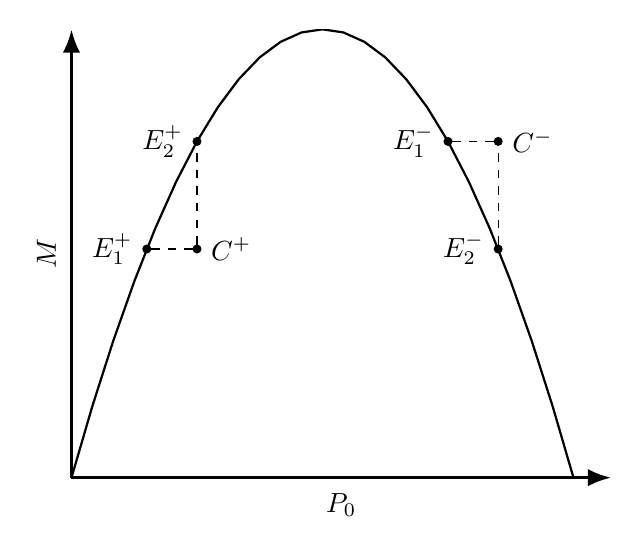
\begin{tikzpicture}
%\begin{axis}[axis x line=bottom, axis y line=left, xlabel=$P_0$, ylabel=$M$, xtick=\empty, ytick=\empty]
\begin{axis}[axis x line=bottom, axis y line=left, axis line style={very thick, -Latex[]}, xlabel=$P_0$, ylabel=$M$, xtick=\empty, ytick=\empty, xmax=1.15]
	\addplot[thick, domain=-1:+1, black] {-x^2};

	\node (E1inc) [draw=black, circle, fill, inner sep=1pt, label=left:$E_1^+$] at (axis cs:-0.7,-0.49) {};
	\node (E2inc) [draw=black, circle, fill, inner sep=1pt, label=left:$E_2^+$] at (axis cs:-0.5,-0.25) {};
	\node  (Cinc) [draw=black, circle, fill, inner sep=1pt, label=right:$C^+$ ] at (axis cs:-0.5,-0.49) {};

	\node (E1dec) [draw=black, circle, fill, inner sep=1pt, label=left:$E_2^-$] at (axis cs:+0.7,-0.49) {};
	\node (E2dec) [draw=black, circle, fill, inner sep=1pt, label=left:$E_1^-$] at (axis cs:+0.5,-0.25) {};
	\node  (Cdec) [draw=black, circle, fill, inner sep=1pt, label=right:$C^-$ ] at (axis cs:+0.7,-0.25) {};

	\draw [dashed] (E1inc) -- (Cinc) -- (E2inc);
	\draw [dashed] (E1dec) -- (Cdec) -- (E2dec);
\end{axis}
\end{tikzpicture}
\caption{\label{fig:nstars:stability_mass_pressure}%
	Suppose an equilibrium star $E_1^+$ on an \emph{increasing} part of the mass-pressure curve $M(P_0)$ is compressed to a non-equilibrium star $C^+$ with the same mass.
	Compared to the \emph{more massive} equilibrium star $E_2^+$ with the increased central pressure, it experiences \emph{less} gravitational attraction, causing it to expand back towards the original equilibrium configuration $E_1^+$.
	In contrast, suppose an equilibrium star $E_1^-$ on a \emph{decreasing} part of the mass-pressure curve is compressed to a non-equilibrium star $C_-$ with the same mass.
	Compared to the \emph{less massive} equilibrium star $E_2^-$ with the increased central pressure, it experiences \emph{more} gravitational attraction, causing it to compress even more and ultimately implode.
}
\end{figure}

A third necessary condition for stars parametrized by their central pressure $P_0$ is
\begin{equation}
	\odv{M(P_0)}{P_0} > 0
	\qquad \text{(necessary condition)} .
\label{eq:nstars:stability_mass_pressure}
\end{equation}
To understand it, consider a star $E_1^+$ in equilibrium on the increasing part of the mass-pressure curve in \cref{fig:nstars:stability_mass_pressure}, where condition \eqref{eq:nstars:stability_mass_pressure} is satisfied.
Now compress this star to the non-equilibrium star $C^+$ with the same mass, and let $E_2^+$ be the star in equilibrium with the same central pressure as $C^+$.
Then $C^+$ has less mass than $E_2^+$, and hence weaker gravitational forces than $E_2^+$, but the same central pressure as $E_2^+$.
As a result, the star will expand and hence decrease its central density and pressure, causing it to return towards the equilibrium star $E_1^+$.

Let us repeat the argument on the decreasing part of the curve, where condition \eqref{eq:nstars:stability_mass_pressure} does not hold.
After the compression from $E_1^-$ to $C^-$, we see that $C^-$ has more mass and hence stronger gravitational forces than $E_2^-$, but again the same central pressure.
The star therefore contracts, and repeating the argument causes it to collapse completely.

The criterion \eqref{eq:nstars:stability_mass_pressure} shows that the stars located between the maximum mass and the bottom of the spiral in \cref{fig:nstars:massradius} are unstable!

\subsection{General analysis of stability}
\label{sec:nstars:stability_general}

The arguments presented above were necessary, but not sufficient for stellar stability.
Let us analyze the stability of the stars in a more rigorous way by finding a mathematical definition \TODO{criterion?} of stability.
We will follow the path of Chandrasekhar \cite{ref:chandrasekhar_stability} and \cite[§ 26.4d]{ref:mtw}.

\subsubsection{Perturbation theory for the fluid displacement}

In \cref{sec:einstein_to_tov}, we showed that in the spherically symmetric metric
\begin{equation}
	\dif s^2 = e^{2 \alpha_0(r)} \dif t^2 - e^{2 \beta_0(r)} \dif r^2 - r^2 \left( \dif \theta^2 + \sin^2 \theta \dif \phi^2 \right) ,
\end{equation}
for a perfect fluid with energy-momentum
\begin{equation}
	T_{\mu \nu} = \frac{1}{c^2} u_\mu u_\nu (\epsilon_0 + P_0) - g_{\mu \nu} P_0
	\qquad \text{where} \qquad
	P_0 = P_0(r) \text{ and } \epsilon_0 = \epsilon_0(r)
\label{eq:nstars:energy_momentum}
\end{equation}
that is in \emph{equilibrium} with four-velocity
\begin{equation}
	u^\mu = (u^0, 0, 0, 0) ,
\label{eq:nstars:velocity_equilibrium}
\end{equation}
the Einstein field equations \eqref{eq:einstein} reduce to
\begin{subequations}%
\begin{align}%
	\frac{1}{r^2} e^{-2 \beta_0} \left( 2 r \beta_0' - 1 + e^{2 \beta_0} \right)  &= \frac{8 \pi G}{c^4} \epsilon_0   && \left( G_{00} = \frac{8 \pi G}{c^4} T_{00} \right) , \label{eq:nstars:field_equations_equilibrium_00} \\
	\frac{1}{r^2} e^{-2 \beta_0} \left( 2 r \alpha_0' + 1 - e^{2 \beta_0} \right) &= \frac{8 \pi G}{c^4} P_0          && \left( G_{11} = \frac{8 \pi G}{c^4} T_{11} \right) , \label{eq:nstars:field_equations_equilibrium_11} \\
	\alpha_0'                                                                     &= \frac{-1}{\epsilon_0 + P_0} P_0' && \left( \nabla_\mu T\indices{^\mu_1} = 0 \right)    , \label{eq:nstars:field_equations_equilibrium_T}
	%e^{-2 \beta_0} \left( \alpha_0'' + (\alpha_0')^2 - \alpha_0' \beta_0' + \frac{1}{r} (\alpha_0' - \beta_0') \right) &= \frac{8 \pi G}{c^4} P_0,
\end{align}%
\label{eq:nstars:field_equations_equilibrium}%
\end{subequations}%
where $' = \pdv{}/{r}$.

Now we suppose that the fluid is no longer in equilibrium, but rather let loose in the radial direction with four-velocity
\begin{equation}
	u^\mu = (u^0, u^1, 0, 0) .
	\quad
\label{eq:nstars:velocity_unstable}
\end{equation}
By the spherical symmetry, we still assume that there is only radial motion of fluid elements.
In a rotating neutron star -- a pulsar -- for example, the situation would be more complicated.
The metric should therefore still be spherically symmetric, but $\alpha_0(r) \rightarrow \alpha(r,t)$ and $\beta_0(r) \rightarrow \beta(r,t)$ are now promoted to time-dependent functions, and therefore so are the pressure $P_0(r) \rightarrow P(r,t)$ and energy density $\epsilon_0(r) \rightarrow \epsilon(r,t)$.
We therefore have the new metric
\begin{equation}
	\dif s^2 = e^{2 \alpha(t, r)} \dif t^2 - e^{2 \beta(t, r)} \dif r^2 - r^2 \left( \dif \theta^2 + \sin^2 \theta \dif \phi^2 \right) .
\label{eq:nstars:metric_unstable}
\end{equation}
To make calculations tractable, we assume that the fluid is only \emph{slightly perturbed} from equilibrium.
Following \cite{ref:chandrasekhar_stability}, let us use perturbation theory and express the new functions
\begin{equation}
\begin{aligned}
	\alpha   (t, r) &= \alpha_0  (r) + \delta \alpha  (t, r), & \qquad \qquad
	P        (t, r) &= P_0       (r) + \delta P       (t, r), \\
	\beta    (t, r) &= \beta_0   (r) + \delta \beta   (t, r), & \qquad \qquad
	\epsilon (t, r) &= \epsilon_0(r) + \delta \epsilon(t, r), \\
\end{aligned}
\label{eq:nstars:perturbation_expansion}
\end{equation}
with small perturbations $\delta \alpha$, $\delta \beta$, $\delta P$ and $\delta \epsilon$ around their equilibrium values and calculate everything only to first order in the small quantities.

We want to determine the displacement of fluid elements from the unperturbed star to the perturbed star.
Evolution of this quantity should give us insight into how the star responds to perturbations.
Let us therefore define $\xi(t, r)$ so that if we attach a tracker to some fixed fluid element in the star, then
\begin{equation}
\begin{split}
	\text{      in the unperturbed star, } & \text{the fluid element is at $\big(ct,r,\theta,\phi\big)$,} \\
	\text{while in the   perturbed star, } & \text{the fluid element is at $\big(ct,r+\xi(r,t),\theta,\phi\big)$.} \\
\end{split}
\end{equation}
Like $\delta \alpha$, $\delta \beta$, $\delta P$ and $\delta \epsilon$, we treat $\xi$ as a small quantity.

What is the relation between the fluid element displacement $\xi(r,t)$ and the fluid's four-velocity?
By our definition, $\pdv{\xi}/{t} = \odv{r}/{t}$, where right side is to be interpreted as the derivative of the fluid element's radial coordinate taken \emph{along its world line} -- or \emph{stream line} -- $x(\tau)$.
The chain rule then gives
\begin{equation}
	\dot\xi = \pdv{\xi}{t} = \odv{r}{t} = \frac{\odv{r}/{\tau}}{\odv{t}/{\tau}} = c \, \frac{u^1}{u^0} .
\end{equation}
We can express $u^0$ and $u^1$ in terms of $\dot\xi$ by combining this equation with the normalization condition $u_\mu u^\mu = e^{2 \alpha} \left( u^0 \right)^2 - e^{2 \beta} \left( u^1 \right)^2 = c^2$.
To first order in $\dot\xi$ and $\delta \alpha$, we find the components
\begin{subequations}
\begin{align}
	u^0 &= \frac{c \, e^{-\alpha}}{\sqrt{1 - \left( e^{\beta-\alpha} \dot\xi / c \right)^2 }} \taylor c \, e^{-\alpha_0} \, (1 - \delta \alpha), \\
	u^1 &= \frac{\dot\xi \, e^{-\alpha}}{\sqrt{1 - \left( e^{\beta-\alpha} \dot\xi / c \right)^2 }} \taylor \dot\xi \, e^{-\alpha_0} .
\end{align}
\label{eq:nstars:velocity_components}
\end{subequations}

In the perturbed system, the field equations \eqref{eq:nstars:field_equations_equilibrium} also change and must be rederived from the Einstein equations \eqref{eq:einstein} in the new metric \eqref{eq:nstars:metric_unstable} subject to the energy-momentum \eqref{eq:nstars:energy_momentum} with the non-equilibrium velocity \eqref{eq:nstars:velocity_unstable}.
As always, the field equations follow from the machinery of \cref{eq:def_christoffel,eq:def_riemann_tensor,eq:def_ricci_tensor,eq:def_ricci_scalar}.
This time we calculate the field equations only to first order in the small quantities and subtract the equilibrium equations \eqref{eq:nstars:field_equations_equilibrium} to simplify them.
The calculation is easy in principle, although in practice perhaps not -- we borrow the results obtained by \cite[§26.4d]{ref:mtw}, who find that two of the new field equations are
\begin{subequations}
\begin{align}
	%\delta \beta   &= - \frac{4 \pi G}{c^4} (\epsilon_0 + P_0) r e^{2 \beta_0} \xi                                                                                                && \left( G_{01} = \frac{8 \pi G}{c^4} T_{01} \right) , \\
	%\delta \alpha' &= \frac{r}{2 e^{-2 \beta_0}} \left[ \frac{8 \pi G}{c^4} \delta P + 2 e^{-2 \beta_0} \left( \frac{2}{r} \alpha_0' + \frac{1}{r^2} \right) \delta \beta \right] && \left( G_{11} = \frac{8 \pi G}{c^4} T_{11} \right) .
	%%\delta \alpha' &= 4 \pi \left\{ -\gamma P_0 \frac{e^{2 \beta_0}}{r} (r^2 e^{-\alpha_0} \xi)' + \left[ P_0' r - (\epsilon_0 + P_0) e^{2 \beta_0} \xi \right] \right\}
	%
	\frac{2}{r} e^{-(\beta_0 + \alpha_0)} \dot{\delta\beta}                                     &= - \frac{8 \pi G}{c^4} (\epsilon_0 + P_0) e^{\beta_0 - \alpha_0} \dot\xi                         && \left( G_{01} = \frac{8 \pi G}{c^4} T_{01} \right) , \\
	\frac{2}{r} e^{-2\beta_0} \left( \delta\alpha' - \alpha_0' - \frac{\delta \beta}{r} \right) &= \phantom{-} \frac{8 \pi G}{c^4} \delta P                                                                    && \left( G_{11} = \frac{8 \pi G}{c^4} T_{11} \right) .
\end{align}
\end{subequations}
We can erase the two dots in the first equation by performing a time integration, forgetting about the integration constant because $\delta\beta=0$ when we are back in equilibrium with $\xi=0$.
The simplest form of the field equations is therefore
\begin{subequations}
\begin{align}
	\frac{1}{r} e^{-2\alpha_0} \delta\beta                                                      &= -           \frac{4 \pi G}{c^4} (\epsilon_0 + P_0) \xi , \label{eq:nstars:field_equations_unstable_01} \\
	\frac{1}{r} e^{-2\beta_0} \left( \delta\alpha' - \alpha_0' - \frac{\delta \beta}{r} \right) &= \phantom{-} \frac{4 \pi G}{c^4} \delta P               . \label{eq:nstars:field_equations_unstable_11}
\end{align}
\Cref{eq:nstars:field_equations_unstable_01,eq:nstars:field_equations_unstable_11} are analogous to \cref{eq:nstars:field_equations_equilibrium_00,eq:nstars:field_equations_equilibrium_11}.
What is the third equation corresponding to \cref{eq:nstars:field_equations_equilibrium_T}, which we found from conservation of energy-momentum $\nabla_\mu T^{\mu \nu} = 0$ back in \cref{sec:einstein_to_tov}?
In \cref{chap:relfluid}, we study relativistic fluid mechanics and start from $\nabla_\mu T^{\mu \nu} = 0$ to derive the relativistic generalization of the Euler equation,
\begin{equation*}
	  \frac{1}{c^2} \Big( \epsilon + P \Big) u^\mu \nabla_\mu u^\alpha = \nabla^\alpha P - \frac{1}{c^2} u^\alpha u^\mu \nabla_\nu P
	  \qquad \left( \nabla_\mu T^{\mu \nu} = 0 \right) .
\end{equation*}
By inserting the new four-velocity components \eqref{eq:nstars:velocity_components} and the expansions \eqref{eq:nstars:perturbation_expansion} into the relativistic Euler equation and performing calculations in the new metric \eqref{eq:nstars:metric_unstable} to first order, \cite[§26.5]{ref:mtw} finds
\begin{equation}
	\left( \epsilon_0 + P_0 \right) e^{2 \beta_0 - 2 \alpha_0} \ddot \xi = -c^2 \left[ \delta P' - \left( \delta \epsilon + \delta P \right) \alpha_0' - \left( \epsilon_0 + P_0 \right) \delta \alpha' \right] .
\label{eq:nstars:field_equations_unstable_T}
\end{equation}%
\label{eq:nstars:field_equations_unstable}%
\end{subequations}%
The system \eqref{eq:nstars:field_equations_unstable} consists of \emph{three} equations for the \emph{five} unknowns $\xi$, $\delta P$, $\delta \epsilon$, $\delta \alpha$ and $\delta \beta$.
To complete the set, we will make use of two further results of our study of relativistic fluid mechanics in \cref{chap:relfluid}.

In order to make use of the results of \cref{chap:relfluid} in our context, we must first learn to distinguish between \emph{Eularian} and \emph{Lagrangian} changes in fluids.
The quantities
\begin{subequations}
\begin{equation}
	\delta f(t, r) = f(t, r) - f_0(r)
\label{eq:nstars:change_eularian}
\end{equation}
that we defined in \cref{eq:nstars:perturbation_expansion} are \textbf{Eularian changes} in the quantities $f$, measured by an observer who is sitting duck at some fixed position $x^\mu = (ct, r, \theta, \phi)$.
In contrast, we define the \textbf{Lagrangian changes}
\begin{equation}
	\Delta f(r,t) = f(r+\xi(r,t), t) - f_0(r)
\label{eq:nstars:change_lagrangian}
\end{equation}
\end{subequations}
as the changes in the same quantities, but measured by an observer who is moving \emph{with} the fluid element as it flows from $r$ to $r + \xi(r,t)$.
One can always be converted into the other through the Taylor expansion
\begin{equation}
\begin{split}
	\Delta f(r,t) &\taylor f(r,t) + \xi(r,t) \, f'(r,t) - f_0(r) \\
	              &= \delta f(r,t) + \xi(r,t) \, f'(r,t) .
\end{split}
\label{eq:nstars:delta_taylor_expansion}
\end{equation}
In words, $\delta$ measures changes at a fixed position but of different fluid elements, while $\Delta$ measures changes of fixed fluid elements but at different positions.
The former stems from our use of perturbation theory, while the latter arises naturally from fluid mechanics.

In our study of relativistic fluid mechanics in \cref{chap:relfluid}, we derive the relativistic generalization \eqref{eq:relfluid:energy_conservation} of conservation of energy in flow of a fluid,
\begin{equation}
	\odv{\epsilon}{\tau} = u^\mu \nabla_\mu \epsilon = -(\epsilon+P) \nabla_\mu u^\mu  .
\label{eq:nstars:energy_conservation}
\end{equation}
First, note that because the equilibrium energy density $\epsilon_0(r)$ is independent of time, $\odv{\epsilon}/{\tau} = \odv{\Delta \epsilon}/{\tau}$.
At first sight, it may sound more straightforward to write $\odv{\delta \epsilon}/{\tau}$ instead of $\odv{\Delta \epsilon}/{\tau}$.
However, since the derivative $\odv{}/{\tau}$ is along the stream line of the fluid element, the Lagrangian changes are more accurate than the Eularian changes to first order in perturbation theory.
To first order in the small quantities, only the time component contributes to the left side
\begin{equation}
\begin{split}
	\odv{\epsilon}{\tau} =
	\odv{\Delta \epsilon}{\tau} =
	u^\mu \nabla_\mu \Delta \epsilon &=
	u^0 \nabla_0 \Delta \epsilon + u^1 \nabla_1 \Delta \epsilon \\
	&\taylor u^0 \pdv{\Delta \epsilon}{t} = u^0 \dot{\Delta \epsilon} =
	e^{-\alpha_0} \dot{\Delta \epsilon} .
\end{split}
\end{equation}
On the right side, we can calculate the quantity $\nabla_\mu u^\mu$ with the identity
\begin{equation}
\begin{split}
	\nabla_\mu u^\mu &= \frac{1}{\sqrt{-\det{g}}} \partial_\mu \left( \sqrt{-g} \, u^\mu \right) \\
	                 &= e^{-\alpha_0} \left[ \dot{\delta\beta} + \frac{e^{-\beta_0}}{r^2} \left( e^{\beta_0} r^2 \dot\xi \right)' \right] .
\end{split}
\end{equation}
To first order in the small quantities, \cref{eq:nstars:energy_conservation} then says
\begin{equation}
	\dot{\Delta \epsilon} = - \left( \epsilon_0 + P_0 \right) \left[ \dot{\delta\beta} + \frac{e^{-\beta_0}}{r^2} \left( e^{\beta_0} r^2 \dot\xi \right)' \right] .
\end{equation}
Again, integrate with respect to time to get rid of the dots and set the integration constant to zero, so $\Delta \epsilon = 0$ when $\delta \beta = 0$ and $\xi = 0$.
We then find our fourth main equation
\begin{equation}
	\Delta \epsilon = - \left( \epsilon_0 + P_0 \right) \left[ \delta\beta + \frac{e^{-\beta_0}}{r^2} \left( e^{\beta_0} r^2 \xi \right)' \right] .
\label{eq:nstars:Delta_epsilon}
\end{equation}

The last result of \cref{chap:relfluid} that we make use of is adiabadicity of the flow.
In \cref{sec:relfluid:adiabadicity}, we show that the flow of a perfect fluid is adiabatic with the \textbf{adiabatic index}
\begin{equation}
	\gamma = \frac{\epsilon+P}{P} \odv{P}{\epsilon} .
\label{eq:nstars:adiabatic_index0}
\end{equation}
The above expression can be calculated entirely from the fluid's equation of state $\epsilon = \epsilon(P)$, although in its current form, it is the \emph{unknown}, perturbed quantities $\epsilon$ and $P$ that enter -- not the known equilibrium quantities $\epsilon_0$ and $P_0$.
However, by interpreting the derivative as the ratio of Lagrangian changes, the adiabatic index can be rewritten in the visually similar, but fundamentally distinct form
\begin{equation}
	\gamma = 
	\frac{\epsilon+P}{P} \frac{\Delta P}{\Delta \epsilon} ,
	\quad \text{or} \quad
	\Delta P = \frac{P}{\epsilon + P} \, \gamma \, \Delta \epsilon .
\label{eq:nstars:adiabatic_index}
\end{equation}
The latter is a relation between two first order \TODO{first-order?} quantities, and so for the purpose of perturbation theory, \emph{the only relevant part of $\gamma$ is the zeroth order \TODO{zeroth order? other places too?} part}
\begin{equation}
	\gamma_0 = \frac{\epsilon_0+P_0}{P_0} \odv{P_0}{\epsilon_0}
	         = \frac{\epsilon_0+P_0}{P_0} \frac{\Delta P_0}{\Delta \epsilon_0} .
\end{equation}
This gives us our fifth and final equation
\begin{equation}
	\Delta P = \frac{P_0}{\epsilon_0 + P_0} \, \gamma_0 \, \Delta \epsilon
	         = \odv{P_0}{\epsilon_0} \, \Delta\epsilon .
\label{eq:nstars:Delta_P}
\end{equation}

We have made quite a big mess by now, but we finally have all the information we need, and it remains only to clean up after ourselves.
Together, equations \eqref{eq:nstars:field_equations_unstable_01}, \eqref{eq:nstars:field_equations_unstable_11}, \eqref{eq:nstars:field_equations_unstable_T}, \eqref{eq:nstars:Delta_epsilon} and \eqref{eq:nstars:Delta_P} constitute the system of five equations
\begin{subequations}
\begin{align}
	\frac{1}{r} e^{-2\alpha_0} \delta\beta                                                      &= -           \frac{4 \pi G}{c^4} (\epsilon_0 + P_0) \xi , \label{eq:nstars:perturbation_system_01} \\
	\frac{1}{r} e^{-2\beta_0} \left( \delta\alpha' - \alpha_0' - \frac{\delta \beta}{r} \right) &= \phantom{-} \frac{4 \pi G}{c^4} \delta P               , \label{eq:nstars:perturbation_system_11} \\
	\left( \epsilon_0 + P_0 \right) e^{2 \beta_0 - 2 \alpha_0} \ddot \xi                                                        &= -c^2 \left[ \delta P' - \left( \delta \epsilon + \delta P \right) \alpha_0' - \left( \epsilon_0 + P_0 \right) \delta \alpha' \right] , \label{eq:nstars:perturbation_system_euler} \\
	\Delta \epsilon                                                                                                             &= - \left( \epsilon_0 + P_0 \right) \left[ \delta\beta + \frac{e^{-\beta_0}}{r^2} \left( r^2 e^{\beta_0} \xi \right)' \right]  , \label{eq:nstars:perturbation_system_energy_conservation} \\
	\Delta P &= \frac{P_0}{\epsilon_0 + P_0} \, \gamma_0 \, \Delta \epsilon = \odv{P_0}{\epsilon_0} \, \Delta\epsilon, \label{eq:nstars:perturbation_system_adiabadicity}
\end{align}%
\label{eq:nstars:perturbation_system}%
\end{subequations}%
for the five unknowns $\xi$, $\delta \alpha$, $\delta \beta$, $\delta P$ and $\delta \epsilon$.
Remember that any occurence of $\Delta P$ and $\Delta \epsilon$ can be traded for $\delta P$ and $\delta \epsilon$ by the Taylor expansion \eqref{eq:nstars:delta_taylor_expansion}.
Except for the independent variables $t$ and $r$, the only other quantities are the equilibrium values $\alpha_0$, $\beta_0$, $P_0$ and $\epsilon_0$ and derivatives thereof.
Solving the Tolman-Oppenheimer-Volkoff equations \eqref{eq:tov:tovsys} yield $P_0$, $m_0$ and $\alpha_0$, from which one can calculate $\epsilon_0$ by the equation of state \eqref{eq:tov:tovsys_eos} and $\beta_0$ from definition \eqref{eq:einstein_to_tov:def_m}.

It is the displacement $\xi(t,r)$ we want to calculate, so let us reduce the system \eqref{eq:nstars:perturbation_system} to a differential equation involving it as the only dependent variable.
Along the way, it is convenient to define
\begin{equation}
	\zeta(t,r) = r^2 e^{\beta_0(r)} \xi(t,r),
\label{eq:nstars:definition_zeta}
\end{equation}
because the only spatial derivative of $\xi$ in the system \eqref{eq:nstars:perturbation_system} appears through this combination in \cref{eq:nstars:perturbation_system_energy_conservation}.
Never forget that we are doing perturbation theory, so we can still neglect any product of two small quantities, and we can simplify expressions using any equilibrium equation from above.
Again, the work before us is easy in principle and hard in practice.
In the end, \cite[equation 26.19]{ref:mtw} find that $\zeta$ obeys the differential equation
\begin{equation}
	W(r) \ddot{\zeta}(r,t) = \left[ \Pi(r) \zeta'(r) \right]' + Q(r) \zeta(r) ,
\label{eq:nstars:diffeq_zeta}
\end{equation}
where the coefficient functions are
\begin{subequations}
\begin{align}
	\Pi &= \frac{1}{r^2} e^{\beta_0 + 3 \alpha_0} \gamma_0 P_0 , \label{eq:nstars:sturm_liouville_coefficients_Pi} \\
	Q   &= -\frac{4}{r^3} e^{\beta_0 + 3 \alpha_0} P_0' - \frac{8 \pi G}{c^4} \frac{1}{r^2} e^{3 \beta_0 + 3 \alpha_0} P (\epsilon_0 + P_0) + \frac{e^{\beta_0 + 3 \alpha_0}}{r^2(\epsilon_0 + P_0)} \left( P_0' \right)^2 , \label{eq:nstars:sturm_liouville_coefficients_Q} \\
	W   &= \frac{1}{c^2 r^2} e^{3 \beta_0 + \alpha_0} (\epsilon_0 + P_0) . \label{eq:nstars:sturm_liouville_coefficients_W}
\end{align}
\label{eq:nstars:sturm_liouville_coefficients}
\end{subequations}
\TODO{final comment?}

\subsubsection{General Sturm-Liouville solution for the fluid displacement}

We can find a solution to the differential equation \eqref{eq:nstars:diffeq_zeta} using separation of variables.
Let us assume a solution of the form
\begin{equation}
	\zeta(t,r) = T(t) \, U(r) .
\label{eq:nstars:separation_of_variables}
\end{equation}
Substituting the trial solution \eqref{eq:nstars:separation_of_variables} into the differential equation \eqref{eq:nstars:diffeq_zeta} and dividing by $W U T$, we see that
\begin{equation}
	\frac{\ddot{T}}{T} = \frac{\left( \Pi \, U' \right)' + Q \, U}{W \, U} = -\omega^2
\end{equation}
must be a constant $-\omega^2$, which can be any complex number at this stage.
We then find the temporal solutions solutions $T(t) = e^{\pm i \omega t}$, while the spatial function $U(r)$ and $\omega^2$ must solve
\begin{equation}
	\odv*{ \left[ \Pi(r) \odv{U(r)}{r} \right] }{r} + \left[ Q(r) + \omega^2 W(r) \right] U(r) = 0 .
\label{eq:nstars:diffeq_U}
\end{equation}

What are the boundary equations for $U(r)$?
At the center $r = 0$, spherical symmetry implies that there can be no flow, so the physical boundary condition there is
\begin{equation}
	\xi(t, 0) = 0.
\label{eq:nstars:boundary_condition_center_physical}
\end{equation}
From definitions \eqref{eq:nstars:definition_zeta} and \eqref{eq:nstars:separation_of_variables}, we see that this requires
\TODO{why not $r^4$, $r^5$, etc? do we need $\xi' > 0$ at $r=0$ or something? dimensional analysis requires $U \propto r^3$?}
\begin{equation}
	U(r) \propto r^3
	\qquad \text{near } r = 0.
\label{eq:nstars:boundary_condition_center_mathematical}
\end{equation}
At the surface $r = R$, there can be no change in pressure as one follows a fluid element, just like at the interface between water and air down on Earth.
The boundary condition here is therefore
\begin{equation}
	\Delta P = 0
	\qquad \text{at } r = R.
\label{eq:nstars:boundary_condition_surface_physical}
\end{equation}
\TODO{remark why Lagrangian change!}
From \cref{eq:nstars:perturbation_system_adiabadicity}, we see that this is equivalent to
\begin{equation}
	\Delta P = \odv{P_0}{\epsilon_0} \Delta \epsilon = \left( \frac{v_0}{c} \right)^2 \Delta\epsilon ,
\label{eq:nstars:deltaP_product}
\end{equation}
where we recognize the derivative from the speed of sound $v_0 = c \sqrt{\odv{P_0}/{\epsilon_0}}$.
The surface $r = R$ is defined by $P_0 = 0$, and where there is no pressure, there can be no sound, so we should have $v_0 = 0$.
\TODO{but is not true for conformal limit where $\epsilon = 3 P$ ! write about this here?}
This can be confirmed from the equation of state.
Close to the surface, the pressure \eqref{eq:nstars:pressure_zeroT} is small, so $x_F$ is also small, and it is therefore the non-relativistic equation of state \eqref{eq:nstars:nr_eos} that reigns.
Its derivative is
\begin{equation}
	\odv{\epsilon_0}{P_0} \propto \odv{P_0^{3/5}}{P_0} \propto P_0^{-2/5} = \infty ,
	\qquad \text{so} \qquad
	v_s^2 \propto \odv{P_0}{\epsilon_0} = \frac{1}{\odv{\epsilon_0}/{P_0}} = \frac{1}{\infty} = 0
	\quad \text{at } r = R.
\end{equation}
Hence, the first factor $\odv{P_0}/{\epsilon_0}$ of the product \eqref{eq:nstars:deltaP_product} is zero, and the whole product will vanish \emph{provided that} the second factor $\Delta \epsilon$ is finite.
Glancing back at expression \eqref{eq:nstars:perturbation_system_adiabadicity} for $\Delta \epsilon$, it then follows that the boundary condition \eqref{eq:nstars:boundary_condition_surface_physical} is \emph{automatically} satisfied \emph{provided that}
\begin{equation}
	\Delta \epsilon = - \left( \epsilon_0 + P_0 \right) \left[ \delta\beta + \frac{e^{-\beta_0(R)}}{R^2} U'(R) e^{i \omega t} \right] \quad \text{is finite}.
\end{equation}
By assumption, $\delta\beta$ is a small and thus finite quantity, and $e^{-\beta_0(R)} = \left( 1 - 2 G M / R c^2 \right)^{-1/2}$ is also finite.
The translation of the boundary condition \eqref{eq:nstars:boundary_condition_surface_physical} at the surface into a criterion on $U(r)$ is therefore only that
\begin{equation}
	\odv{U(r)}{r} \quad \text{is finite} \quad \text{at } r = R.
\label{eq:nstars:boundary_condition_surface_mathematical}
\end{equation}

\TODO{first \emph{now} i introduce $U_n$, multiple solutions, etc. Make sure this is logical}
The differential equation \eqref{eq:nstars:diffeq_U} subject to the boundary conditions \eqref{eq:nstars:boundary_condition_center_mathematical} and \eqref{eq:nstars:boundary_condition_surface_mathematical} is a \textbf{Sturm-Liouville problem} for eigenfunctions $U(r) = U_n(r)$ and their corresponding eigenvalues $\omega^2 = \omega_n^2$.
It is best viewed as the eigenvalue equation
\begin{subequations}
\begin{align}
	&\odv*{ \left[ \Pi(r) \odv{U_n(r)}{r} \right] }{r} + Q(r) \, U_n(r) = -\omega_n^2 W(r) U_n(r) && \text{for } 0 \leq r \leq R , \label{eq:nstars:sturm_liouville} \\
	\text{subject to} \quad & U_n(r)          \propto r^3    && \text{near } r=0 , \label{eq:nstars:sturm_liouville_boundary_condition1} \\
	\text{and}        \quad & \odv{U_n(r)}{r} <       \infty && \text{at } r=R . \label{eq:nstars:sturm_liouville_boundary_condition2}
\end{align}%
\label{eq:nstars:sturm_liouville_problem}%
\end{subequations}
In the form above, the Sturm-Liouville equation is expressed in a self-adjoint form with respect to the inner product
\begin{equation}
	\braket{f | g} = \int_0^R \dif r \, f(r) g(r) .
\label{eq:nstars:function_inner_product}
\end{equation}
Denoting the left side by $\hat{L} U_n = \hat{L}(r) U_n(r)$, we can integrate by parts twice to show that for two solutions $U_m(r)$ and $U_n(r)$,
\begin{equation}
\begin{split}
	\Braket{\hat{L} U_m | U_n} &= \int_0^R \dif r \, \left[ \left( \Pi U_m' \right)' U_n + Q U_m U_n \right] \\
	                           &= \Big[ \Pi U_m' U_n \Big] + \int_0^R \dif r \, \Big[ - \Pi U_m' U_n' + Q U_m U_n \Big] \\
	                           &= \Big[ \Pi U_m' U_n \Big] - \Big[ \Pi U_m U_n' \Big] + \int_0^R \dif r \, \Big[ \left( \Pi U_n' \right)' U_m + Q U_m U_n \Big] \\
	                           &= \Big[ \Pi \, U_m' \, U_n \Big]_{r=0}^{r=R} - \Big[ \Pi \, U_m \, U_n' \Big]_{r=0}^{r=R} + \Braket{U_m | \hat{L} U_n} . \\
\end{split}
\end{equation}
The surface terms at $r = 0$ vanish because $U_n(0) = U_m(0) = 0$ there by boundary condition \eqref{eq:nstars:boundary_condition_center_mathematical}, while the surface terms at $r = R$ vanish because $P_0(R) = 0$ there, causing $\Pi(R) = 0$ from its definition \eqref{eq:nstars:sturm_liouville_coefficients_Pi}.
Using the inner product \eqref{eq:nstars:function_inner_product} and the property 
\TODO{need to say that the functions are \emph{real}!}
\begin{equation}
	\braket{\hat{L} U_m | U_n} = \braket{U_m | \hat{L} U_n}
\label{eq:nstars:inner_product_hermitean}
\end{equation}
that follows, one can dive into the field of Sturm-Liouville theory, where one will discover the following important properties:
\begin{subequations}
\begin{enumerate}
\item \label{item:nstars:sturm_liouville_eigenvalues} The eigenvalues $\omega_n^2$ are real and form an infinite, discrete sequence
\begin{equation}
	\omega_0^2 < \omega_1^2 < \omega_2^2 < \cdots
\end{equation}
that is bounded from below, but not from above.

The proof of reality is within our reach.
Applying property \eqref{eq:nstars:inner_product_hermitean} with $U_m = U_n$, we have $\braket{\hat{L} U_n | U_n} = \conj{\braket{\hat{L} U_n | U_n}}$.
Exchanging the left side of $\hat{L} U_n = -\omega_n^2 W U_n$ with the right and noting that $\braket{W U_n | U_n}$ is real, this is equivalent to $-\omega_n^2 \braket{W U_n | U_n} = \conj{\left( -\omega_n^2 \right)} \braket{W U_n | U_n}$, so $\omega_n^2$ is real.
Proving the last part takes more work, but we will that it plays out in practice when solving the Sturm-Liouville problem numerically soon.

\item \label{item:nstars:sturm_liouville_zeros} The eigenfunction $U_n(r)$ corresponding to the eigenvalue $\omega_n^2$ has exactly
\begin{equation}
	n \text{ zeros } U_n(r) = 0 \quad \text{for} \quad 0 < r < R .
\end{equation}
Intuitively, by rewriting the Sturm-Liouville equation as $\left( \Pi U_n' \right)' / U_n = - \left( Q + \omega_n^2 W \right)$ and noting that $W > 0$ by its definition \eqref{eq:nstars:sturm_liouville_coefficients_W}, it is apparent that as $\omega_n^2$ increases, so does the oscillatory behavior of $U_n$ around $U_n = 0$, and hence the number of zeros.

\item \label{item:nstars:sturm_liouville_completeness} Eigenfunctions $U_n(r)$ corresponding to different eigenvalues $\omega_n^2$ are different, and constitute an orthonormal basis for the Hilbert space of functions on $[0, R]$ \TODO{what functions? real? smooth?} with respect to the $W$-weighted inner product 
\begin{equation}
	\braket{U_m | U_n}_W = \braket{W U_m | U_n} = \delta_{m n} .
\end{equation}
We can give a quick proof of the first part.
Property \eqref{eq:nstars:inner_product_hermitean} implies that $-\omega_n^2 \braket{W U_n  | U_m} = -\omega_m^2 \braket{W U_m | U_n}$, so $\left( \omega_m^2 - \omega_n^2 \right) \braket{W U_m | U_n} = 0$.
If $U_m = U_n$ are equal, then $\braket{W U_m | U_n} \neq 0$, so $\omega_m^2 = \omega_n^2$ must be equal.
On the other hand, if $\omega_m^2 \neq \omega_n^2$, then $\braket{W U_m | U_n} = 0$, and $U_m \neq U_n$ must be different.
\end{enumerate}
\end{subequations}
\TODO{are the remarks/miniproofs after the statements distracting?}

For an excellent to-the-point overview of Sturm-Liouville theory and rigorous proofs of all the properties, we recommend \TODO{ref to some mathematics text for proofs}.
It can also be comforting to think of a perhaps more familiar example of applied Sturm-Liouville theory, namely the time independent Schrödinger equation $\left[ \left(-\hbar^2/2m\right)\odv[2]{}/{x} + V(x) \right] \psi_n(x) = E_n \psi_n(x)$. \TODO{time-independent?} 
Here, the energies $E_n$ play the role of the eigenvalues $\omega_n^2$ and the wave functions $\psi_n(x)$ are analogous to the eigenfunctions $U_n(r)$.
In one dimension, normalizable solutions to the Schrödinger equation possess precisely the same three properties as above.

\subsubsection{Definition of stellar stability}

At long last, we are now in position to state a rigorous mathematical criterion of stellar stability.
Property \ref{item:nstars:sturm_liouville_completeness} implies that any physically reasonable displacement $\xi(t,r)$ can be written as a linear combination
\begin{equation}
	\xi(t,r) = \frac{e^{-\beta_0(r)}}{r^2} \sum_n c_n U_n(r) e^{i \omega_n t}
\label{eq:nstars:displacement_general_solution}
\end{equation}
for some constants $c_n$.
The superposition will still satisfy the physical boundary conditions \eqref{eq:nstars:boundary_condition_center_physical} and \eqref{eq:nstars:boundary_condition_surface_physical}, provided that each $U_n(r)$ separately satisfies the boundary conditions \eqref{eq:nstars:boundary_condition_center_mathematical} and \eqref{eq:nstars:boundary_condition_surface_mathematical}.
Property \ref{item:nstars:sturm_liouville_eigenvalues} ensures all $\omega_n^2$ are real, \emph{but there is no restriction on the sign of $\omega_n^2$}.

\begin{itemize}
\item If $\omega_0^2 > 0$, then all vibration modes have real frequencies $\omega_n > 0$.
      Then all terms in the displacement \eqref{eq:nstars:displacement_general_solution} merely oscillate back and forth like $\xi \propto e^{i \omega_n t}$, so the star attempts to return to equilibrium, and we say it is \textbf{stable}.
\item If $\omega_0^2 < 0$, then one or more vibration modes have imaginary frequencies $\omega_n = \pm i \abs{\omega_n}$.
      Then some term in the displacement \eqref{eq:nstars:displacement_general_solution} takes off expnentially like $\xi \propto e^{\pm \abs{\omega_n} t}$, so the star either implodes or explodes, and we say it is \textbf{unstable}.
\end{itemize}
A prerequisite for the above definition is that it is sufficient for \emph{one} mode in the displacement \eqref{eq:nstars:displacement_general_solution} to be unstable for the star as a whole to be unstable.
To understand this, suppose a star is exposed to some external perturbation $\xi(t,r)$.
Whatever the source of this perturbation -- be it the touch of a finger, an imperfection in the star's material or the blast from a nearby supernova explosion -- it is the initial state $\xi(t,r)$ of this \emph{external} perturabtion that determines the contribution $c_n$ from each mode in the sum \eqref{eq:nstars:displacement_general_solution}, and subsequently the \emph{response} of the star to the perturbation.
In the real world, we expect that any external perturbation will activate \emph{all} modes $U_n(r)$ to some extent -- for one would need remarkable finger precision to perturb the star in an \emph{exact} superposition of only a finite selection of modes.
Given that all modes have even the slightest nonzero contribution $c_n \neq 0$, the presence of \emph{any} exponential term is sufficient for the whole sum to collapse or grow unbounded towards $0$ or $\infty$.

\TODO{innvending 1: vi gjør perturbasjonsteori, hvorfor er eksponensiell tidsvekst gyldig også når stjernen har blitt veldig mye større/mindre? Svar: kan gjøre flere successive perturbasjoner i små steg!}

\TODO{can the instability stuff be connect to attractor/chaos stuff from nonlinear dynamics? Svar: check fixed points from nonlinear dynamics, check stability by checking the sign of the jacobian matrix or something?}

\TODO{write $\delta r$ instead of $\xi$ to be consistent with the $\delta$-quantities?}

\subsubsection{Numerical solution of the Sturm-Liouville problem with the shooting method}

Multiple methods for determining the stability of stars through our definition above are catalogued by \cite{ref:stability_methods}.
The \textbf{shooting method} is a particularly fun numerical technique for finding the eigenfunctions $U_n(r)$ and eigenvalues $\omega_n^2$ of the Sturm-Liouville problem \eqref{eq:nstars:sturm_liouville_problem}.
Let us put it to use and determine the stability of the stars along the curve in \cref{fig:nstars:massradius}.

\begin{figure}
\begin{tikzpicture}
\pgfplotstableread{../code/data/shoot.dat}{\shoottable}
\pgfplotstablegetrowsof{\shoottable}
\pgfmathparse{int(\pgfplotsretval-1)}
\pgfplotstablegetelem{\pgfmathresult}{r}\of{\shoottable}
\pgfmathsetmacro{\maxR}{\pgfplotsretval}
\begin{axis}[
	width=15cm, height=10cm,
	xlabel=$r/R$, ylabel=$U(r) / \norm{U_0(r)}_\infty$,
	title={Convergence of $U(r) \rightarrow U_0(r)$ as $\omega^2 \rightarrow \omega_0^2$ with the shooting method},
	%every axis title/.style={at={(0.5,1)}, align=center, above=1ex, text width=0.8*\pgfkeysvalueof{/pgfplots/width}]},
	xmin=0, xmax=1, ymin=-2.0, ymax=+2.0,
	xtick distance=0.25, minor x tick num=4,
	ytick distance=2, minor y tick num=3, ymajorgrids,
	cycle list name=color list,
	legend style={anchor=north, at={(0.5, -0.25)}},
	legend columns=8, transpose legend,
	legend cell align=right,
	colormap name=blackred, cycle list={[samples of colormap=32]},
	clip mode=individual,
]
%\addlegendimage{empty legend}
%\addlegendentry{\hspace{-0.6cm}\textbf{Value of $\omega^2$}} % hack for legend title: https://tex.stackexchange.com/questions/2311/add-a-legend-title-to-the-legend-box-with-pgfplots
\pgfplotsinvokeforeach{0,...,31}{ % 31, it works but it is very slow
	\pgfmathparse{int(100 * (0.0 + 0.6 * #1 / 31))} % lin interp 50 -> 100
	\pgfmathsetmacro{\clrintensity}{\pgfmathresult}
	\pgfplotstablegetelem{#1}{nn}\of{\shoottable}
	\ifthenelse{\equal{\pgfplotsretval}{1}}{
		\edef\mycolor{black!\clrintensity!red}
	}{
		\edef\mycolor{black!\clrintensity!blue}
	}
	\edef\temp{\noexpand\addplot+ [thick, color=\mycolor, restrict y to domain=-5:5] table [x expr=\noexpand\thisrow{r}/\maxR, y expr={\noexpand\thisrow{U#1} / 0.000312}] {../code/data/shoot.dat};} % faster to read directly from file for some reason
	\temp
	%\addplot+ [thick, restrict y to domain=-5:5] table [x expr=\thisrow{r}/\maxR, y expr={\thisrow{U#1} / 0.000312}] {../code/data/shoot.dat}; % faster to read directly from file for some reason
	\pgfplotstablegetelem{#1}{omega2}\of{\shoottable} % get value of \omega^2
	\addlegendentryexpanded{$\pgfmathprintnumber[precision=10, fixed, fixed zerofill]{\pgfplotsretval}$}; % pgfplotsretval is still omega2
}
\node [text=black, anchor=north] at (axis description cs:0.5,-0.15) {Value of $\hat{\omega}^2 = \omega^2 / (c/r_0)^2$};
%\addplot [forget plot, dashed, domain=0:5, restrict y to domain=0:2.0, samples=50] {(x*\maxR)^3 / 0.000312} node[pos=0.6, label={[xshift=+0ex]135:$\propto r^3$}] {};
\addplot [forget plot, dashed, domain=0:0.2, restrict y to domain=0:2, samples=100] {700*x^3} node[pos=0.6, label={[xshift=+1ex]135:$\propto r^3$}] {};
\end{axis}
\end{tikzpicture}
\caption{\label{fig:nstars:shooting_convergence}%
	The shooting method finds the eigenvalue $\omega_n^2$ and corresponding eigenfunction $U_n(r)$ with $n=0$ of a Sturm-Liouville problem \eqref{eq:nstars:sturm_liouville_problem}.
	It guesses the eigenvalue $\omega^2$, imposes the boundary condition \eqref{eq:nstars:sturm_liouville_boundary_condition1} near $r = 0$, ``shoots'' across to $r=R$ by integrating the differential equation \eqref{eq:nstars:sturm_liouville} and checks whether $U(r)$ ``hits'' boundary condition \eqref{eq:nstars:sturm_liouville_boundary_condition2} there.
	Based on the number of nodes $n(\omega^2)$ of $U(r)$, the guess is intelligently improved and the process repeated, arriving ever closer to the true eigenvalue $\omega_n^2$.
	First, the algorithm establishes two bounds $\hat{\omega}_-^2 = -16$ and $\hat{\omega}_+^2 = 0$ whose corresponding solutions have $n(\omega_-^2) \leq n$ and $n(\omega_+^2) > n$ nodes.
	The exact squared frequency is then guaranteed to lie in $\omega_-^2 < \omega_n^2 < \omega_+^2$.
	Next, the algorithm finds the number of nodes corresponding to $\hat{\omega}^2 = (\hat{\omega}_-^2 + \hat{\omega}_+^2) / 2 = -8$.
	Here, it is found to have $n(\omega^2) > n$ nodes, so the process is repeated with the tighter upper bound $\hat{\omega}_+^2 = -8$.
	In the opposite case $n(\omega^2) \leq n$, $-8$ would rather be a better lower bound $\hat{\omega}_-^2$.
	The algorithm continues to split the $[\omega_-^2, \, \omega_+^2]$ in this fashion until the bounds are so close that any value in the interval is satisfactory.
	In the plot, \textcolor{blue}{blue} lines correspond to \textcolor{blue}{lower bounds $\omega_-^2$}, \textcolor{red}{red} lines to \textcolor{red}{upper bounds $\omega_+^2$}, brighter colors to initial guesses and darker colors to later guesses.
}
\end{figure}

\usetikzlibrary{calc}
\usepgfplotslibrary{colorbrewer}
\pgfplotsset{cycle list/Dark2} % or Dark2
\begin{figure}
\centering
\begin{tikzpicture}
\pgfplotstableread{../code/data/nmodes_norm.dat}{\nmodestable};
\pgfplotstablegetrowsof{\nmodestable}
\pgfmathparse{int(\pgfmathresult-1)}
\pgfplotstablegetelem{\pgfmathresult}{r}\of{\nmodestable}
\pgfmathsetmacro{\maxR}{\pgfplotsretval}
\begin{groupplot}[
	group style={group size=1 by 2, horizontal sep=5pt, vertical sep=5pt},
	width=15cm, height=9.5cm,
	xmin=-0.0, xmax=1.0, ymin=-1.1, ymax=+1.1, restrict y to domain=-50:+50,
	xtick={0,0.25,0.5,0.75,1}, ytick={-1,0,1},
	ymajorgrids=true,
	%cycle list name=Dark2,%no markers, cycle list name=color list, % or exotic
	cycle multi list={
		solid, dashed\nextlist
		Dark2 % or Set1
	},
]
\nextgroupplot[
	every axis title/.style={at={(0.03,0.07)}, text width=5cm, anchor=south west, draw=black, fill=white},
	title={\subcaption{\label{fig:nstars:modes_normed_separate}Separate normalization}},
	ylabel=$U_n / \norm{U_n}_\infty$,
	legend cell align=left, legend columns=3, legend style={at={(0.5, 1.03)}, anchor=south},
	xticklabels={},
]
\pgfplotsinvokeforeach{0,1,...,7} {
	\addplot+ [thick] table [x expr=\thisrow{r}/\maxR, y=U#1] {\nmodestable};
	\pgfplotstablegetelem{#1}{omega2}\of{\nmodestable}
	\addlegendentryexpanded{$\omega_{#1}^2 = \pgfmathprintnumber[fixed, fixed zerofill, precision=2, showpos=true]{\pgfplotsretval} \, (c / r_0)^2$};
}

\nextgroupplot[
	every axis title/.style={at={(0.97,0.07)}, text width=5cm, anchor=south east, draw=black, fill=white},
	title={\subcaption{\label{fig:nstars:modes_normed_common}Common normalization}},
	xlabel=$r / R$,
	ylabel=$U_n / \norm{U_0}_\infty$,
];
\tablemaximum{../code/data/nmodes.dat}{U0}{\maxU}{r}{\maxr}
\pgfplotsinvokeforeach{0,1,...,7} {
	\addplot+ [thick] table [x expr=\thisrow{r}/\maxR, y expr=\thisrow{U#1}/\maxU] {../code/data/nmodes.dat};
}
\addplot [dashed, domain=0:0.5, restrict y to domain=0:1.1, samples=50] {(x*\maxR)^3 / \maxU} node[pos=0.6, label={[xshift=+0ex]135:$\propto r^3$}] {};
\end{groupplot}
\end{tikzpicture}
\caption{\label{fig:nstars:modes}%
The eight lowest vibration modes $U_n(r)$ and squared eigenfrequencies $\omega_n^2$ for a cold neutron star with central pressure $P = \SI{3e2}{} \epsilon_0$.
In \subref{fig:nstars:modes_normed_separate}, the eigenfunctions are separately normalized to their own maxima, making their shape throughout the star and the boundary condition $U_n(R) < \infty$ clear.
In \subref{fig:nstars:modes_normed_common}, they are instead normalized to a common scale, highlighting the boundary condition $U_n(r) \propto r^3$ for $r \rightarrow 0$.
Here, $r_0 = \SI{10}{\kilo\meter}$.
}
\end{figure}

We describe the shooting method and our implementation of it in detail in \cref{sec:numerics:shooting_method}.
It is also possible to understand the gist of the shooting method from \cref{fig:nstars:shooting_convergence}, where we show how it establishes $\omega_0^2$ and $U_0(r)$ by an intelligent form of ``trial and error''.
In \cref{fig:nstars:modes}, we display the five lowest modes obtained with the shooting method for some star.

Finally, we use the shooting method to examine the stability of every star along the curve in \cref{fig:nstars:massradius}.
For every star, we repeatedly apply the shooting method for $n = 0, \, 1, \, 2, \, \ldots$ to find all negative eigenvalues $\omega_n^2 < 0$ until we encounter the first positive value $\omega_n^2 > 0$.
We then simply count the number of unstable modes with $\omega_n^2 < 0$ and display this number in \cref{fig:nstars:stability}.
The results are very interesting.
\begin{enumerate}
\item Starting from the lowest central pressure, and hence lowest central energy and mass densities, all stars are \emph{stable} up until the maximum mass.
      The part on this segment with lowest central energy density is the territory of Newtonian theory, where we should already expect stars to be stable, but that the situation remains so as relativistic effects take over is not necessarily obvious.
\item At the point of maximum mass, stars gain \emph{one unstable mode}, and the number stays constant as we follow the curve down to the point of the spiral with minimal mass.
      From the necessary stability condition \eqref{eq:nstars:stability_mass_pressure}, we already know that stars on this segment should indeed be unstable.
\item Beyond the spiral's point of minimal mass, stars have a \emph{second unstable mode}.
\item In the innermost parts of the spiral after the next local mass maximum, there even seems to be some stars with a \emph{third unstable mode}.
      The effect is not as crystal clear as it is with the previous segments, however.
\end{enumerate}

Our computations suggest that at every local mass extremum point where $\odv{M(P_0)}/{P_0} = 0$, stars acquire one additional unstable vibration mode, starting with zero unstable modes for the lowest pressures $P_0 \rightarrow 0$.
In fact, \cite{ref:stability_methods} presents a method for determining stability of stars based on this principle!
For a sequence of \emph{cold} stars -- like ours -- in a mass-radius diagram like \cref{fig:nstars:massradius}, the following holds:
\begin{itemize}
\item For the lowermost central energy densities $\epsilon(P_0)$, we know from classical theory that stars are \emph{stable}.
\item At every local mass extremum $\odv{M(P_0)}/{P_0} = 0$ where the curve bends \emph{counterclockwise} as the central pressure increases, one \emph{stable} mode becomes \emph{unstable}.
\item At every local mass extremum $\odv{M(P_0)}/{P_0} = 0$ where the curve bends \emph{clockwise} as the central pressure increases, one \emph{unstable} mode becomes \emph{stable}.
\end{itemize}
Our curve only includes a spiral turning counterclockwise and seem consistent with the first two rules.
We have no spiral turning clockwise, however, and thus no grounds to support nor deny the third rule. \TODO{just drop saying this?}
\cite{ref:stability_rules_thorne} gives a detailed discussion and proofs of these three rules.
As with the Buchdal bound \eqref{eq:incompressible_star:buchdal} that we looked at a long time ago, the maximum mass is not only a limit on \emph{massiveness}, but also on \emph{stability}.
\TODO{can I really say this? I never drew a parametrical mass-radius curve for stars of constant radius, so maybe I should go back and do that}


\usetikzlibrary{decorations.markings}
\begin{figure}[b]
\centering
\pgfplotsset{
	/pgfplots/colormap={stability}{rgb255=(65,171,93) rgb255=(254,178,76) rgb255=(252,78,42) rgb255=(122,1,119)}
}
\begin{tikzpicture}
\begin{groupplot}[
	group style={group size=1 by 1, vertical sep=10pt},
	width=15cm, height=12cm,
	xlabel=$R / \si{\kilo\meter}$, ylabel=$M / \solarmass$,
	grid=major,
	colormap={signnegpos}{samples of colormap=(4 of stability)}, colormap access=const, 
	point meta=explicit, point meta min=0, point meta max=4,
	every axis title/.style={at={(0.97,0.95)}, text width=3cm, anchor=north east, draw=black, fill=white},
	xmin=0, xmax=50, ymin=0, ymax=0.8,
]
\nextgroupplot[
	%title={\subcaption{\label{fig:nstars:stability_computed}Computed}},
	colorbar horizontal, colorbar sampled, colorbar style={xlabel={Number of unstable modes with $\omega_n^2 < 0$}, xtick={0.5, 1.5, 2.5, 3.5}, xticklabels={$0$, $1$, $2$, $3$}, at={(0.5,1.05)}, anchor=south, xticklabel pos=upper, tickwidth=0},
	%xticklabels=\empty,
	minor x tick num=4, minor y tick num=9,
]
\addplot [mesh, very thick] table [x expr={10*\thisrow{R}}, y=M, meta=nu] {../code/data/gr2.dat}
node [text=black, sloped, pos=0.66, yshift=10pt] {$\longleftarrow$ Increasing $P_0$};

% decorate does not work with mesh, so redraw for arrows only!
%\addplot [draw=none, very thick, decoration={markings, mark=between positions 0.05 and 0.85 step 0.2 with {\arrow[scale=1.5]{stealth}}}, postaction=decorate] table [x expr={10*\thisrow{R}}, y=M, meta=nu] {../code/data/gr2.dat}

\iffalse % Exact results are now extremely similar to computed results
\nextgroupplot[
	title={\subcaption{\label{fig:nstars:stability_exact}Exact}},
	xlabel=$R / \si{\kilo\meter}$,
]
\addplot [mark=none, mesh, thick] table [x expr={10*\thisrow{R}}, y=M, meta expr={greater(\thisrow{P},0.8) + greater(\thisrow{P},600) + greater(\thisrow{P},19000)}] {../code/data/gr2.dat};
\fi
\end{groupplot}
\end{tikzpicture}

\caption{\label{fig:nstars:stability}%
Stability analysis of the neutron stars with arbitrary Fermi momenta in \cref{fig:nstars:massradius}.
Squared eigenfrequencies $\omega_n^2$ of the Sturm-Liouville problem \eqref{eq:nstars:sturm_liouville_problem} are computed numerically with shooting method.
The sign of the squared eigenfreuqency $\omega_0^2$ of the lowest normal vibration mode determines whether a star is stable and oscillates like $e^{i \omega_0 t}$, or if it is unstable and grows or decays like $e^{\pm \abs{\omega_0} t}$.
Here, the number of unstable modes with negative squared eigenfrequencies $\omega_n^2 < 0$ are counted for all stars along the mass-radius curve.
\emph{Do note the presence of all four colors.}
}

\end{figure}

\TODO{keywords: $dp/d\epsilon = 1/3$ = conformal limit? no mass in this EOS = scale invariance. $T^{\mu \nu}$ traceless?}
